\documentclass[10pt,a4paper]{article}
\usepackage[utf8]{inputenc}
\usepackage[italian]{babel}
\usepackage{amsmath}
\usepackage{amsfonts}
\usepackage{amssymb}
\usepackage{graphicx}
\usepackage[left=2cm,right=2cm,top=2cm,bottom=2cm]{geometry}

\author{Gruppo 1G.BT \\ Francesco Sacco, Lorenzo Cavuoti}
\title{Es03B: Amplificatore a transistor}

\begin{document}
\maketitle
\paragraph{2) Montaggio del circuito e verifica del punto di lavoro}
\newline
Usando il multimetro digitale abbiamo misurato i valori delle resistenze e condensatori staccati dal circuito
\begin{itemize}
\item $R_1=(178.5\pm1.4)k\Omega$ 
\item $R_2=(17.65\pm0.14)k\Omega$ 
\item $R_C=(9.82\pm0.08)k\Omega$ 
\item $R_E=(1.014\pm0.008)k\Omega$
\item $C_{in}=(221\pm9)nF$
\item $C_{out}=(111\pm4)nF$
\end{itemize}
\\
\subparagraph{a.}
Accendendo soltanto il generatore di ddp continua $V_{CC}=(19.97\pm0.10)$ abbiamo calcolato e misurato il punto di lavoro del transistor che risulta:
\begin{itemize}
\item $V_{CE,att}^Q = (7.3\pm0.4)V \quad$ $I_{C,att}^Q = (1.17\pm0.03)mA \quad$
\item $V_{CE,mis}^Q = (9.00\pm0.05)V \quad$ $ I_{C,mis}^Q = (1.01\pm0.01)mA \quad$
\end{itemize}
I due risultati non sono compatibili, tuttavia, come si vedrà anche in seguito, il circuito funziona correttamente, la discrepanza quindi si potrebbe attribuire a un errore nella presa dati o nei calcoli

\subparagraph{b.}
Usando il multimetro digitale abbiamo misurato le tensioni ai terminali del transistor che risultano:
\begin{itemize}
\item $V_{B,mis} = 1.647\pm0.008 \quad$ $V_{E,mis} = 1.034\pm 0.005 \quad$ $V_{BE,mis} = 0.614\pm0.003 \quad$ $V_{C,mis} = 10.01\pm0.05$
\item $V_{B,att} \approx 1.7 \quad$ $V_{E,att} \approx 1.1 \quad$ $V_{BE,att} = 0.6 \quad$ $V_{C,att} \approx 10$\newline
Purtroppo è stato impossibile dare una stima accurata degli errori a causa dell'incognita su alcuni parametri del transistor
\end{itemize}
\subparagraph{c.}
Sfruttando l'effetto transistor con $h_{fe}\approx 100$ abbiamo $I_B = I_C/h_{fe} \approx 10.1 \mu A$ dove $I_C$ è stata calcolata vedendo la ddp ai capi di $R_C$, inoltre sappiamo che $I_B = I_1-I_2 = (9\pm2)\mu A$ con $I_1$, $I_2$ calcolate prendendo la ddp su $R_1$, $R_2$ rispettivamente. L'errore risulta grande il quanto differenza di due misure simili, infatti $I_1=102.2\pm1.4\mu A$ $I_2=93.1\pm1.3\mu A$. Le due misure risultano compatibili, l'errore su 
	
\paragraph{3) Risposta a segnali sinusoidali a frequenza fissa}
In questo punto colleghiamo il generatore di funzioni al circuito con $f=6.24kHz$ e tutti i voltaggi sono misurati picco-picco
\subparagraph{i}
Vedendo $V_{in}$ e $V_{out}$ accoppiando l'oscilloscopio in AC notiamo che i due segnali sono in controfase con uno circa 10 volte l'altro (figura \ref{screen})
\begin{figure}
\centering
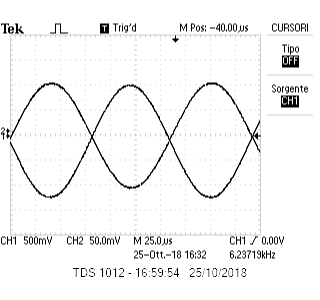
\includegraphics[scale=1]{3_1.png}
\caption{Inversione di fase tra ingresso e uscita, si notino le diverse scale su CH1 e CH2}
\label{screen} 
\end{figure}

\subparagraph{ii}
Il guadagno atteso per piccoli segnali risulta $A_{V,att}=9.68\pm0.14$, per un onda sinusoidale con $V_{in} = (0.22\pm0.01)V$ si ha $V_{out} = (2.06\pm0.09)V$, $A_V=9.3\pm0.6$. Per verificare la linearità del sistema abbiamo preso un onda triangolare a diverse ampiezze. Con $V_{in} = (0.22\pm0.01)V$ si ha $V_{out} = (1.98\pm0.09V)$ $A_V=9.1\pm0.6$ e, con $V_{in} = 1.51\pm0.06V$  triangolare si ha $V_{out} = 13.7\pm0.6V$ $A_V=9.1\pm0.6$ i guadagni attesi risultano compatibili con quelli misurati.\newline
Inoltre la forma d'onda è rimasta pressocchè inalterata, quindi tutte le armoniche dello spettro della triangolare hanno trasformato allo stesso modo, questo dimostra la linearità del circuito tra $1$kHz e $10$kHz.\newline
\subparagraph{iii-iv}
Il circuito risulta lineare per $V_{in}$ minore di circa $1.5 V$ quindi $V_{out} \approx 18 V$ oltre questa ddp si ha il clipping, inizialmente questo spiana l'onda ma alzando ancora di più il voltaggio l'onda si inarca all'interno. 
\end{enumerate}		

\paragraph{4) Risposta in frequenza}
\subparagraph{a}
Abbiamo valutato la risposta in frequenza del circuito per segnali sinusoidali di ampiezza $V_{in}=1V$ e frequenza compresa tra circa 10Hz e 1MHz, cercando di prendere abbastanza punti nelle zone dove il logaritmo del guadagno risulta lineare, cosi' da poter fare 3 fit delle rette che approssimano il guadagno a bassa, media e alta frequenza. I dati raccolti sono riportati in tabella \ref{tab:frequenza}, l'errore su $V_{in}$ e $V_{out}$ è dato dall'incertezza di misura con i cursori dell'oscilloscopio mentre l'errore su $A_V=V_{out}/V_{in}$ è stato fatto propagando l'errore sul rapporto considerando le due misure indipendenti

    \begin{table}[scale=0.8]
        \centering
        \begin{tabular}{ccccccc}
        \hline
            $f [Hz]$& $V_{in} [V]$& $\sigma V_{in} [V]$& $V_{out} [V]$& $\sigma V_{out} [V]$& $A_V$& $\sigma A_V$&
            \hline
            13.7& 1.00& 0.04& 2.72& 0.12& 2.72& 0.17&
            16.3& 1.00& 0.04& 3.02& 0.13& 3.02& 0.19&
            47.0& 1.00& 0.04& 6.3& 0.3& 6.3& 0.4&
            68.1& 1.00& 0.04& 7.4& 0.3& 7.4& 0.5&
            98.4& 1.00& 0.04& 8.2& 0.4& 8.2& 0.5&
            118& 1.00& 0.04& 8.6& 0.4& 8.6& 0.6&
            213& 1.00& 0.04& 9.2& 0.4& 9.2& 0.6&
            565& 1.00& 0.04& 9.3& 0.4& 9.3& 0.6&
            1.18 k& 1.00& 0.04& 9.4& 0.4& 9.4& 0.6&
            2.11 k& 1.00& 0.04& 9.4& 0.4& 9.4& 0.6&
            11.7 k& 1.00& 0.04& 9.4& 0.4& 9.4& 0.6&
            20.3 k& 1.00& 0.04& 9.0& 0.4& 9.0& 0.6&
            71.3 k& 1.00& 0.04& 7.3& 0.3& 7.3& 0.4&
            209 k& 1.00& 0.04& 3.74& 0.16& 3.7& 0.2&
            739 k& 1.00& 0.04& 1.14& 0.05& 1.14& 0.07&
            2.10 M& 1.00& 0.04& 0.40& 0.02& 0.40& 0.03&
        \end{tabular}
        \caption{Dati della risposta in frequenza del circuito}
        \label{tab:frequenza}
    \end{table}

\subparagraph{b}
Abbiamo riportato i dati in un diagramma di bode ed eseguito tre fit lineari con la funzione curve-fit del modulo scipy di python usando absolute-sigma=False, gli errori sulle frequenze si sono trascurati in quanto il loro prodotto per la derivata della funzione è molto minore degli errori sul guadagno (1\% vs 5-6\%). La funzione di fit utilizzata è$f(x)=a*x+b$, i tre fit presentano: 
\begin{itemize}
\item $a=13.8\pm0.2$, $b=-7.01\pm0.3$, $\chi^2=0.029$ Per le basse frequenze
\item $a=0.084\pm0.3$, $b=19.12\pm0.08$, $\chi^2=0.019$ Per le medie frequenze
\item $a=-19.3\pm0.3$, $b=114\pm2$, $\chi^2=0.19$ Per le alte frequenze
\end{itemize}

Il $\chi^2$ risulta molto minore delle aspettative, probabilmente dovuto a una sovrastima dell'incertezza sulla misura delle tensioni con l'oscilloscopio

\begin{figure}
	\centering
    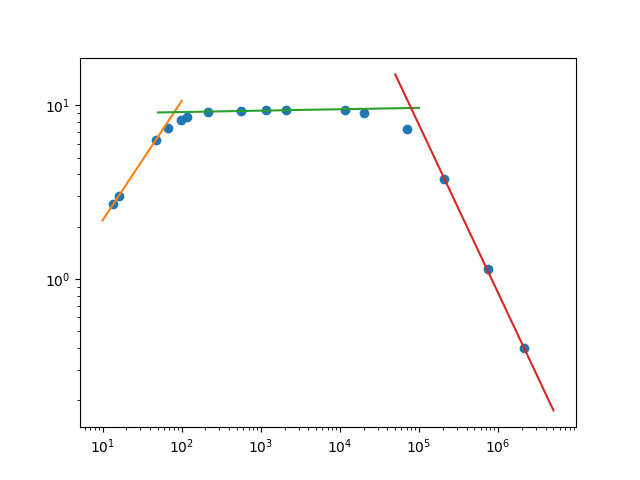
\includegraphics[scale=0.8]{fit.png} 
    \caption{Grafico di bode del circuito}
    \label{fig:fit}
\end{figure}
    
\subparagraph{c}
Analizzando il circuito possiamo notare che $C_{in}$ e $R_2//R_1$ compongono un filtro passa alto, inoltre il transistor ha una piccola capacità interna che con $R_C$ forma un filtro passa basso, la frequenza si nota solo per frequenze elevate agendo da passa basso. Dal fit otteniamo $F_L=81\pm2 Hz$ e $F_H=81\pm3 kHz$
		
\end{document}